\documentclass[article]{uom-coursework}
% \usepackage[showframe]{geometry}

\usetikzlibrary{automata, positioning, arrows,
arrows.meta}

\usepackage{float}
\usepackage{syntax}

\usepackage{etoolbox}% http://ctan.org/pkg/etoolbox
\makeatletter
\patchcmd{\lst@GLI@}% <command>
  {\def\lst@firstline{#1\relax}}% <search>
  {\def\lst@firstline{#1\relax}\def\lst@firstnumber{#1\relax}}% <replace>
  {\typeout{listings firstnumber=firstline}}% <success>
  {\typeout{listings firstnumber not set}}% <failure>
\makeatother

\counterwithout{section}{chapter}

\lstset{inputpath={../src}, numbers=left,
language=C++}

\newcommand{\listref}[1]{Listing~\ref{lst:#1}}

% Biblography
% \addbibresource{dsa.bib}

\title{Compiler Theory and Practice}
\tagline{Coursework}
\author{Juan Scerri}
\authorid{123456A}
\courseworkname{Some Degree}
\doctype{coursework}
\courseworkdate{\monthyeardate\today}
\subjectcode{CPS2000}


\begin{document}

%----------------------------------
%	Front Matter
%----------------------------------

\pagestyle{umpage}

\frontmatter

\maketitle % Print the title page

\tableofcontents % Print the table of contents

\clearpage

\lstlistoflistings

\clearpage

\mainmatter

\chapter*{Report}
\label{chap:report}
\addcontentsline{toc}{chapter}{\nameref{chap:report}}

\section{Lexer}

\subsection{Design \& Implementation}

The lexer was split into three-main components. A
DFSA class, a generic table-driven lexer, and a
lexer builder.

\subsubsection{The DFSA}

The DFSA class is an almost-faithful
implementation of the formal concept of a DFSA.
\listref{dfsadecl}, outlines the behaviour of the
DFSA. Additionally it contains a number of helper
functions which facilitate getting the initial
state and checking whether a state or a transition
category is valid. These helpers specifically,
\texttt{getInitialState()} is present since after
building the DFSA there is no guarantee the
initial state used by the user will be the same.

\lstinputlisting[
firstline=14,
lastline=44,
caption={DFSA Class Declaration (lexer/DFSA.hpp)},
label=lst:dfsadecl
]{lexer/DFSA.hpp}

The only significant difference is the
\texttt{getTransition()} functions. In fact, it
accepts a vector of transition categories instead
of a single category.

This is because a symbol e.g. `\texttt{a}',
`\texttt{9}' etc, might be valid for multiple
categories. For instance `\texttt{a}` is
considered to be both a letter and a number in
hexadecimal.

The DFSA for accepting the micro-syntax
\texttt{PArL} is built as follows.

Let $\mathfrak{U}$ be the set of all possible
characters under the system encoding (e.g. UTF-8).

The will use the following categories:

\begin{itemize}
    \item $L \coloneq \{
        \texttt{A},\ldots,\texttt{Z},\texttt{a},\ldots,\texttt{z}\}$
    \item $D \coloneq
        \{\texttt{0},\ldots,\texttt{9}\}$
    \item $H \coloneq
        \{\texttt{A},\ldots,\texttt{F},\texttt{a},\ldots,\texttt{f}\}
        \cup D$
    \item $S \coloneq \{\alpha \in \mathfrak{U}
        \colon \alpha\ \text{is
    whitespace}\}\setminus\{\texttt{LF}\}$
\end{itemize}

Note: \texttt{LF} refers to line-feed or as it is
more commonly known `\texttt{\textbackslash n}'
i.e. new-line.

Together these categories form our alphabet
$\Sigma$:

$$\Sigma \coloneq L \cup D \cup S \cup
\{\texttt{.},\texttt{\#},\texttt{\_},\texttt{(},\texttt{)},\texttt{[},\texttt{]},\texttt{\{},\texttt{\}},\texttt{*},\texttt{/},\texttt{+},\texttt{-},\texttt{<},\texttt{>},\texttt{=},\texttt{!},\texttt{,},\texttt{:},\texttt{;},\texttt{LF}\}$$

Now, the following drawing describe the
transitions of the DFSA. For improved readability
the DFSA has been split across mulitple drawings.
Hence, in each drawing  initial state $0$ refers
to the \emph{same} initial state (a DFSA has one
and only one initial state).

Additionally, each final state is annotated with
the token type it should produce.

\tikzset{
node distance=2cm, % specifies the minimum distance between two nodes. Change if necessary.
every state/.style={thick, fill=gray!10}, % sets the properties for each ’state’ node
initial text=$\text{start}$, % sets the text that appears on the start arrow
}

\begin{figure}[H]
\centering
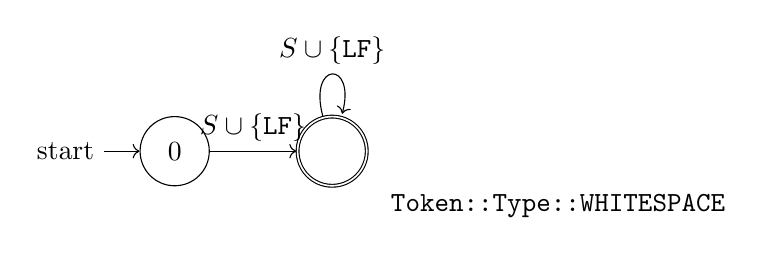
\begin{tikzpicture}
\node[state,initial] (q1) {$0$};
\coordinate[right of=q1] (tq1) {};
\node[state, right of=tq1, accepting] (q2) {};
\node [below right = 0.1cm and 0.3cm of q2]
    {\texttt{Token::Type::WHITESPACE}};
\draw
    (q1) edge[above, ->] node{$S\cup\{\texttt{LF}\}$} (q2)
    (q2) edge[loop above, ->] node{$S\cup\{\texttt{LF}\}$} (q2);
\end{tikzpicture}
\caption{States \& transitions for recognising
whitespace}
\end{figure}

\begin{figure}[H]
\centering
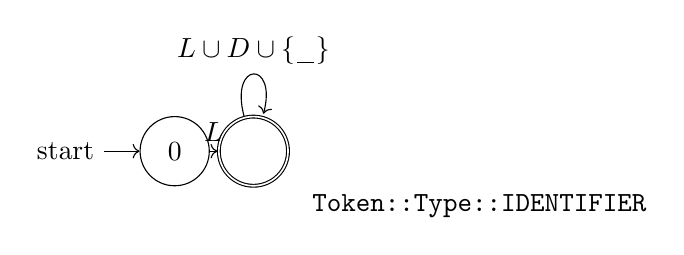
\begin{tikzpicture}
\node[state,initial] (q1) {$0$};
\node[state, right of=q1, accepting] (q2) {};
\node [below right = 0.1cm and 0.3cm of q2]
    {\texttt{Token::Type::IDENTIFIER}};
\draw
    (q1) edge[above, ->] node{$L$} (q2)
    (q2) edge[loop above, ->] node{$L \cup D \cup \{\texttt{\_}\}$} (q2);
\end{tikzpicture}
\caption{States \& transitions for recognising
identifiers/keywords}
\end{figure}

\begin{figure}[H]
\centering
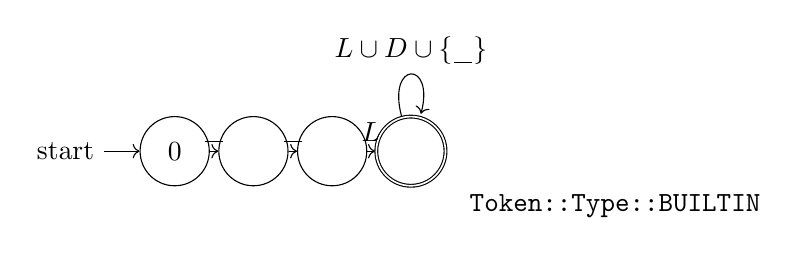
\begin{tikzpicture}
\node[state,initial] (q1) {$0$};
\node[state, right of=q1] (q2) {};
\node[state, right of=q2] (q3) {};
\node[state, right of=q3, accepting] (q4) {};
\node [below right = 0.1cm and 0.3cm of q4]
    {\texttt{Token::Type::BUILTIN}};

\draw
    (q1) edge[above, ->] node{\texttt{\_}} (q2)
    (q2) edge[above, ->] node{\texttt{\_}} (q3)
    (q3) edge[above, ->] node{$L$} (q4)
    (q4) edge[loop above, ->] node{$L \cup D \cup \{\texttt{\_}\}$} (q4);
\end{tikzpicture}
\caption{States \& transitions for recognising
builtins}
\end{figure}


\begin{figure}[H]
\centering
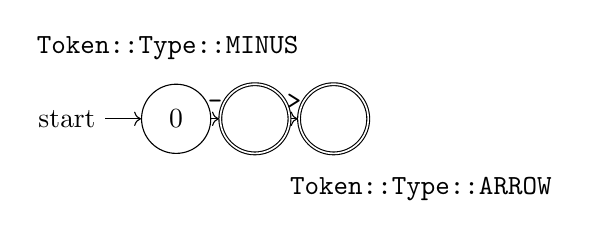
\begin{tikzpicture}
\node[state,initial] (q1) {$0$};
\node[state, right of=q1, accepting] (q2) {};
\node[state, right of=q2, accepting] (q3) {};
\node [above left = 0.3cm and -1cm of q2]
    {\texttt{Token::Type::MINUS}};
\node [below right = 0.3cm and -1cm of q3]
    {\texttt{Token::Type::ARROW}};
\draw
    (q1) edge[above, ->] node{\texttt{-}} (q2)
    (q2) edge[above, ->] node{\texttt{>}} (q3);
\end{tikzpicture}
\caption{States \& transitions for recognising
minus and arrow (\texttt{->})}
\end{figure}

\begin{figure}[H]
\centering
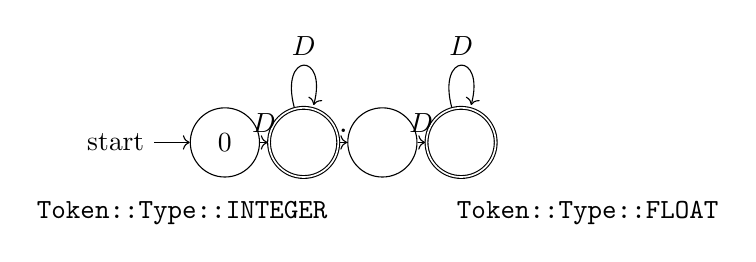
\begin{tikzpicture}
\node[state,initial] (q1) {$0$};
\node[state, right of=q1, accepting] (q2) {};
\node[state, right of=q2] (q3) {};
\node[state, right of=q3, accepting] (q4) {};
\node [below left = 0.3cm and -0.75cm of q2]
    {\texttt{Token::Type::INTEGER}};
\node [below right = 0.3cm and -0.5cm of q4]
    {\texttt{Token::Type::FLOAT}};
\draw
    (q1) edge[above, ->] node{$D$} (q2)
    (q2) edge[loop above, ->] node{$D$} (q2)
    (q2) edge[above, ->] node{\texttt{.}} (q3)
    (q3) edge[above, ->] node{$D$} (q4)
    (q4) edge[loop above, ->] node{$D$} (q4)
    ;
\end{tikzpicture}
\caption{States \& transitions for recognising
integers and floats}
\end{figure}

\begin{figure}[H]
\centering
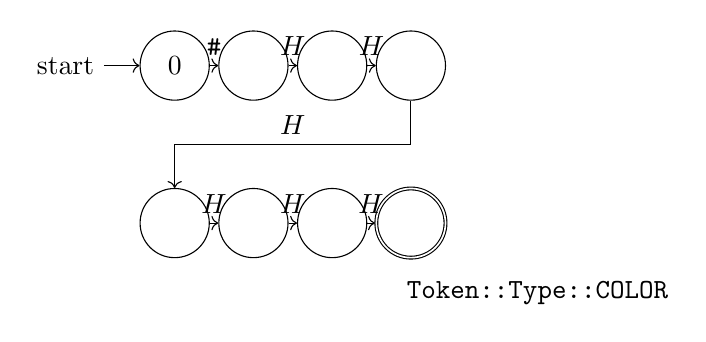
\begin{tikzpicture}
\node[state,initial] (q1) {$0$};
\node[state, right of=q1] (q2) {};
\node[state, right of=q2] (q3) {};
\node[state, right of=q3] (q4) {};

\coordinate[below of=q1] (bq1) {};
\coordinate[below of=q4] (bq4) {};

\node[state, below of=bq1] (q5) {};
\node[state, right of=q5] (q6) {};
\node[state, right of=q6] (q7) {};
\node[state, right of=q7, accepting] (q8) {};
\node [below right = 0.3cm and -0.5cm of q8]
    {\texttt{Token::Type::COLOR}};
\draw
    (q1) edge[above, ->] node{\texttt{\#}} (q2)
    (q2) edge[above, ->] node{$H$} (q3)
    (q3) edge[above, ->] node{$H$} (q4)
    (q4) -- (bq4)
    (bq4) edge[above] node{$H$} (bq1)
    (bq1) edge[->] (q5)
    (q5) edge[above, ->] node{$H$} (q6)
    (q6) edge[above, ->] node{$H$} (q7)
    (q7) edge[above, ->] node{$H$} (q8)
    ;
\end{tikzpicture}
\caption{States \& transitions for recognising
colours}
\end{figure}

\begin{figure}[H]
\centering
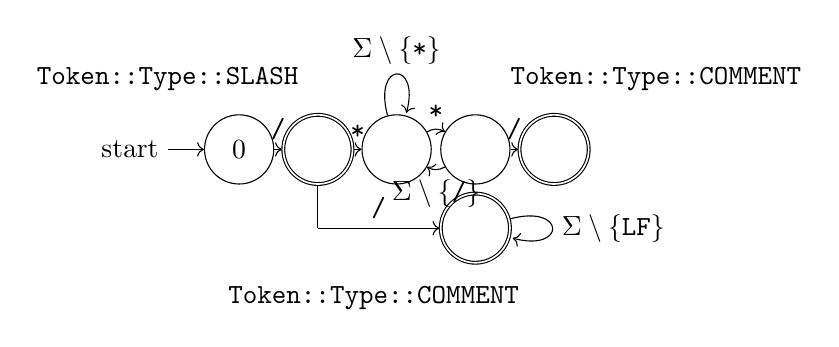
\begin{tikzpicture}
\node[state,initial] (q1) {$0$};
\node[state, right of=q1,accepting] (q2) {};

\coordinate[below of=q2] (bq2) {};

\node[state, right of=q2] (q4) {};
\node[state, right of=q4] (q5) {};
\node[state, right of=q5,accepting] (q6) {};

\node[state, below of=q5, accepting] (q3) {};

\node [above left = 0.3cm and -0.2cm of q2]
    {\texttt{Token::Type::SLASH}};

\node [above right = 0.3cm and -1cm of q6]
    {\texttt{Token::Type::COMMENT}};

\node [below left = 0.3cm and -1cm of q3]
    {\texttt{Token::Type::COMMENT}};

\draw
    (q1) edge[above, ->] node{\texttt{/}} (q2)
    (q2) -- (bq2)
    (bq2) edge[above, ->] node{\texttt{/}} (q3)
    (q3) edge[loop right, ->] node{$\Sigma \setminus \{\texttt{LF}\}$} (q3)
    (q2) edge[above, ->] node{\texttt{*}} (q4)
    (q4) edge[loop above, ->] node{$\Sigma \setminus \{\texttt{*}\}$} (q4)
    (q4) edge[above, bend left, ->] node{\texttt{*}} (q5)
    (q5) edge[below, bend left, ->] node{$\Sigma \setminus \{\texttt{/}\}$} (q4)
    (q5) edge[above, ->] node{\texttt{/}} (q6)
    ;
\end{tikzpicture}
\caption{States \& transitions for recognising
slashes and comments}
\end{figure}

\begin{figure}[H]
\centering
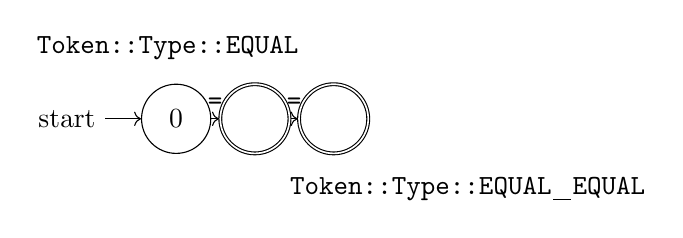
\begin{tikzpicture}
\node[state,initial] (q1) {$0$};
\node[state, right of=q1, accepting] (q2) {};
\node[state, right of=q2, accepting] (q3) {};
\node [above left = 0.3cm and -1cm of q2]
    {\texttt{Token::Type::EQUAL}};
\node [below right = 0.3cm and -1cm of q3]
    {\texttt{Token::Type::EQUAL\_EQUAL}};
\draw
    (q1) edge[above, ->] node{\texttt{=}} (q2)
    (q2) edge[above, ->] node{\texttt{=}} (q3);
\end{tikzpicture}
\caption{States \& transitions for assign
and is equal to}
\end{figure}

\begin{figure}[H]
\centering
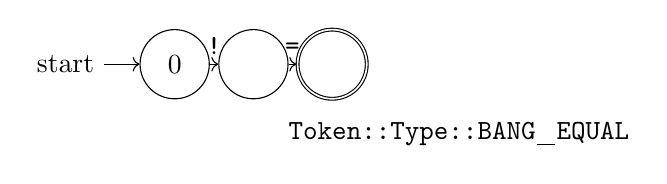
\begin{tikzpicture}
\node[state,initial] (q1) {$0$};
\node[state, right of=q1] (q2) {};
\node[state, right of=q2, accepting] (q3) {};
\node [below right = 0.3cm and -1cm of q3]
    {\texttt{Token::Type::BANG\_EQUAL}};
\draw
    (q1) edge[above, ->] node{\texttt{!}} (q2)
    (q2) edge[above, ->] node{\texttt{=}} (q3);
\end{tikzpicture}
\caption{States \& transitions for not equal to}
\end{figure}


\begin{figure}[H]
\centering
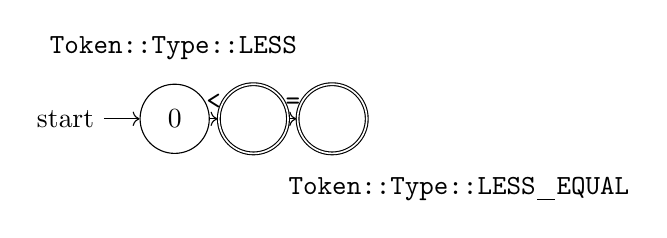
\begin{tikzpicture}
\node[state,initial] (q1) {$0$};
\node[state, right of=q1, accepting] (q2) {};
\node[state, right of=q2, accepting] (q3) {};
\node [above left = 0.3cm and -1cm of q2]
    {\texttt{Token::Type::LESS}};
\node [below right = 0.3cm and -1cm of q3]
    {\texttt{Token::Type::LESS\_EQUAL}};
\draw
    (q1) edge[above, ->] node{\texttt{<}} (q2)
    (q2) edge[above, ->] node{\texttt{=}} (q3);
\end{tikzpicture}
\caption{States \& transitions for less than
and less than or equal to}
\end{figure}

\begin{figure}[H]
\centering
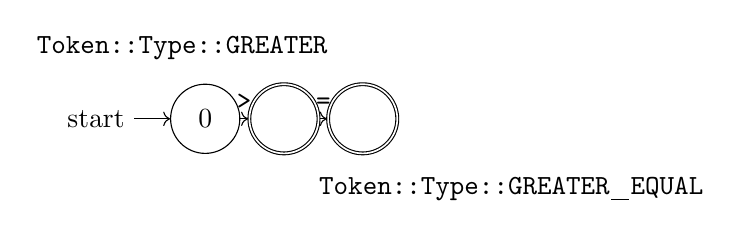
\begin{tikzpicture}
\node[state,initial] (q1) {$0$};
\node[state, right of=q1, accepting] (q2) {};
\node[state, right of=q2, accepting] (q3) {};
\node [above left = 0.3cm and -1cm of q2]
    {\texttt{Token::Type::GREATER}};
\node [below right = 0.3cm and -1cm of q3]
    {\texttt{Token::Type::GREATER\_EQUAL}};
\draw
    (q1) edge[above, ->] node{\texttt{>}} (q2)
    (q2) edge[above, ->] node{\texttt{=}} (q3);
\end{tikzpicture}
\caption{States \& transitions for greater than
and greater than or equal to}
\end{figure}


\begin{figure}[H]
\centering
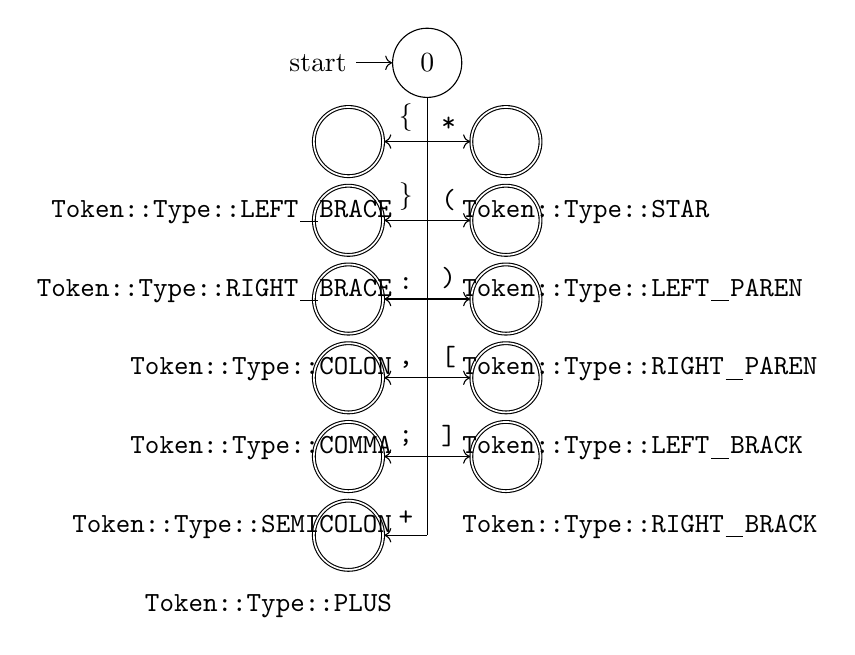
\begin{tikzpicture}
\node[state,initial] (q1) {$0$};

\coordinate[below of=q1] (b1) {};
\coordinate[below of=b1] (b2) {};
\coordinate[below of=b2] (b3) {};
\coordinate[below of=b3] (b4) {};
\coordinate[below of=b4] (b5) {};
\coordinate[below of=b5] (b6) {};

\node[state, right of=b1, accepting] (q2) {};
\node[state, below of=q2, accepting] (q3) {};
\node[state, below of=q3, accepting] (q4) {};
\node[state, below of=q4, accepting] (q5) {};
\node[state, below of=q5, accepting] (q6) {};

\node[state, left of=b1, accepting] (q7) {};
\node[state, below of=q7, accepting] (q8) {};
\node[state, below of=q8, accepting] (q9) {};
\node[state, below of=q9, accepting] (q10) {};
\node[state, below of=q10, accepting] (q11) {};
\node[state, below of=q11, accepting] (q12) {};

\node [below right = 0.3cm and -1cm of q2]
    {\texttt{Token::Type::STAR}};
\node [below right = 0.3cm and -1cm of q3]
    {\texttt{Token::Type::LEFT\_PAREN}};
\node [below right = 0.3cm and -1cm of q4]
    {\texttt{Token::Type::RIGHT\_PAREN}};
\node [below right = 0.3cm and -1cm of q5]
    {\texttt{Token::Type::LEFT\_BRACK}};
\node [below right = 0.3cm and -1cm of q6]
    {\texttt{Token::Type::RIGHT\_BRACK}};

\node [below left = 0.3cm and -1cm of q7]
    {\texttt{Token::Type::LEFT\_BRACE}};
\node [below left = 0.3cm and -1cm of q8]
    {\texttt{Token::Type::RIGHT\_BRACE}};
\node [below left = 0.3cm and -1cm of q9]
    {\texttt{Token::Type::COLON}};
\node [below left = 0.3cm and -1cm of q10]
    {\texttt{Token::Type::COMMA}};
\node [below left = 0.3cm and -1cm of q11]
    {\texttt{Token::Type::SEMICOLON}};
\node [below left = 0.3cm and -1cm of q12]
    {\texttt{Token::Type::PLUS}};

\draw
    (q1) -- (b1)
    (b1) -- (b2)
    (b2) -- (b3)
    (b3) -- (b4)
    (b4) -- (b5)
    (b5) -- (b6)
    ;

\draw
    (b1)  edge[above, ->] node{\texttt{*}} (q2)
    (b2) edge[above, ->] node{\texttt{(}} (q3)
    (b3) edge[above, ->] node{\texttt{)}} (q4)
    (b4) edge[above, ->] node{\texttt{[}} (q5)
    (b5) edge[above, ->] node{\texttt{]}} (q6)

    (b1) edge[above, ->] node{\texttt{\{}} (q7)
    (b2) edge[above, ->] node{\texttt{\}}} (q8)
    (b3) edge[above, ->] node{\texttt{:}} (q9)
    (b4) edge[above, ->] node{\texttt{,}} (q10)
    (b5) edge[above, ->] node{\texttt{;}} (q11)
    (b6) edge[above, ->] node{\texttt{+}} (q12)
    ;
\end{tikzpicture}
\caption{States \& transitions for single letter tokens}
\end{figure}

\subsubsection{The Builder \& Director}

Each sequence of states present is directly
represented in code within the
\texttt{LexerDirector} using methods provided by
the \texttt{LexerBuilder}.

\lstinputlisting[
firstline=297,
lastline=309,
caption={Code specification of
the comments in the \texttt{LexerDirector}
(lexer/LexerDirector.cpp)},
label=lst:commenttransitions
]{lexer/LexerDirector.cpp}

The \texttt{LexerBuilder} keeps track of these
transitions using less efficient data structures
such as hash maps (\texttt{std::unordered\_map})
and sets (\texttt{std::unordered\_set}).

Then the \texttt{build()} method processes the
user defined transitions and normalises everything
into a single transition table for use in a DFSA.
Additionally, it also produces two other
artefacts. The first is called
\texttt{categoryIndexToChecker}. It is a hash map
from the index of a category to a lambda function
which takes a character as input and returns true
or false.

The lambdas and the category indices are also
registered by the user. See \listref{checkerreg}
for a registration example. Additionally, the
category indices although they are integers for
readability they are defined as an enumeration.

\lstinputlisting[
firstline=51,
lastline=58,
caption={Registration of the hexadecimal category
checker (lexer/LexerDirector.cpp)},
label=lst:checkerreg
]{lexer/LexerDirector.cpp}

The second artefact produced by the builder is
also a hash map from final states to their
associated token type.

The transition table is then passed onto the DFSA.
And the DFSA, and the two artefacts are passed
onto the Lexer class.

\lstinputlisting[
firstline=210,
lastline=224,
caption={Constructions of the Lexer
(lexer/LexerBuilder.cpp)},
]{lexer/LexerBuilder.cpp}

\subsubsection{The Actual Lexer}

The lexer's core is as was described during the
lectures and the core/main method is
\texttt{simulateDFSA()}.

It also has a number of very important auxiliary
methods and behavioural changes. Specifically, the
\texttt{updateLocationState()}, see
\listref{updateloc}, is critical for providing
adequate error messages both during the current
stage and for later stages. This function is
called every time a lexeme is consumed allowing
the lexer to keep track of where in the file it
is, in terms of lines and columns.

\lstinputlisting[
firstline=110,
lastline=122,
caption={The \texttt{updateLocationState()} lexer
method (lexer/Lexer.cpp)},
label=lst:updateloc
]{lexer/Lexer.cpp}

Additionally, if an invalid / non-accepting state
is reached the invalid lexeme is consumed and the
user is warned, see \listref{lexererrors}. After
this the lexer, is left in a still operational state.
Hence, \texttt{nextToken()} can be used again.

 This is critical to provide users of the
 \texttt{PArL} compiler with a list of as many
 errors as possible, since it would be a bad
 experience to have to constantly run the
 \texttt{PArL} compiler to see the next error.

\lstinputlisting[
firstline=56,
lastline=84,
caption={Error handling mechanism in the
\texttt{nextToken()} lexer method
(lexer/Lexer.cpp)},
label=lst:lexererrors
]{lexer/Lexer.cpp}

\subsubsection{Hooking up the Lexer to the Runner}

The \texttt{Runner} class is the basic structure
which connects all the stages of the
compiler together together.

In this case the Runner passes in a reference to
the lexer into the parser, this allows the parser
to request tokens and they are computed on demand
improving overall performance. Additionally, this
has the benefit of allowing the parsing of larger
and multiple files since, the parser is no longer
limited by the amount of usable memory, since it
does not need to load the whole file.

However, in this case no such optimisation is
present.

\lstinputlisting[
firstline=22,
lastline=28,
caption={The Runner constructor passes
\texttt{mLexer} into the Parser constructor
(runner/Runner.cpp)}
]{runner/Runner.cpp}

\section{The AST \& Parsing}

\subsection{Modified EBNF}

\setlength{\grammarparsep}{8pt plus 1pt minus 1pt} % increase separation between rules
\setlength{\grammarindent}{10em} % increase separation between LHS/RHS

Some modifications were applied to the original EBNF. Some of
the modifications were either motivated by improved user
experience, a more uniform mechanism and others to reduce
complexity further down the pipeline.

\begin{center}
\begin{grammar}
<Letter> ::= `A'-`Z' | `a'-`z'

<Digit> ::= `0'-`9'

<Hex> ::= `A'-`F' | `a'-`F' | <Digit>

<Identifier> ::= <Letter> \{`\_' | <Letter> | <Digit>\}

<BooleanLiteral> ::= `true' | `false'

<IntegerLiteral> ::= <Digit> \{<Digit>\}

<FloatLiteral> ::= <Digit> \{<Digit>\} `.' <Digit> \{<Digit>\}

<ColorLiteral> ::= `\#' <Hex> <Hex> <Hex> <Hex> <Hex> <Hex>

<ArrayLiteral> ::= `[' [<Epxr> \{`,' <Epxr>\}] `]'

<PadWidth> ::= `\_\_width'

<PadHeight> ::= `\_\_height'

<PadRead> ::= `\_\_read' <Epxr> `,' <Epxr>

<PadRandomInt> ::= `\_\_random\_int' <Epxr>

<Literal> ::= <BooleanLiteral>
\alt <IntegerLiteral>
\alt <FloatLiteral>
\alt <ColorLiteral>
\alt <ArrayLiteral>
\alt <PadWidth>
\alt <PadHeight>
\alt <PadRead>
\alt <PadRandomInt>

<Type> ::= (`bool' | `int' | `float' | `color') [ `[' <IntegerLiteral> `]' ]

<SubEpxr> ::= `(' <Epxr> `)'

<Variable> ::= <Identifier>

<ArrayAccess> ::= <Identifier> `[' <Epxr> `]'

<FunctionCall> ::= <Identifier> `(' [<Epxr> \{`,' <Epxr>\}] `)'

<Epxr> ::= <LogicOr> [`as' <Type>]

<LogicOr> ::= <LogicAnd> \{`or' <LogicAnd>\}

<LogicAnd> ::= <Equality> \{`and' <Equality>\}

<Equality> ::= <Comparison> \{(`==' | `!=') <Comparison>\}

<Comparison> ::= <Term> \{(`<' | `<=' | `>' | `>=') <Term>\}

<Term> ::= <Factor> \{(`+' | `-') <Factor>\}

<Factor> ::= <Unary> \{(`*' | `/') <Unary>\}

<Unary> ::= (`-' | `not') <Unary> | <Primary>

<Primary> ::= <Literal>
\alt <SubExpr>
\alt <Variable>
\alt <ArrayAccess>
\alt <FunctionCall>

<Program> ::= \{<Stmt>\}

<Stmt> ::= <Block>
\alt <VaribaleDecl> `;'
\alt <FunctionDecl>
\alt <Assignment> `;'
\alt <PrintStmt> `;'
\alt <DelayStmt> `;'
\alt <WriteBoxStmt> `;'
\alt <WriteStmt> `;'
\alt <ClearStmt> `;'
\alt <IfStmt>
\alt <ForStmt>
\alt <WhileStmt>
\alt <ReturnStmt> `;'

<Block> ::= `\{' \{<Stmt>\} `\}'

<VariableDecl> ::= `let' <Identifier> `:' <Type> `='
<Epxr>

<FormalParam> ::= <Identifier> `:' <Type>

<FunctionDecl> ::= `fun' <Identifier> `(' [ <ForamlParam>
\{`,' <FormalParam>\}] `)' `->' <Type> <Block>

<Assignment> ::= <Identifier> [`[' <Epxr> `]'] `='
<Epxr>

<PrintStmt> ::= `\_\_print' <Epxr>

<DelayStmt> ::= `\_\_delay' <Epxr>

<WriteBoxStmt> ::= `\_\_write\_box' <Epxr>`,'
<Epxr>`,'<Epxr>`,' <Epxr>`,'<Epxr>

<WriteStmt> ::= `\_\_write' <Epxr>`,' <Epxr>`,'<Epxr>

<ClearStmt> ::= `\_\_clear' <Epxr>

<IfStmt> ::= `if' `(' <Expr> `)' <Block> [`else' <Block>]

<ForStmt> ::= `for' `(' [<VariableDecl>] `;' <Expr> `;'
[<Assignment>] `)' <Block>

<WhileStmt> ::= `while' `(' <Expr> `)' <Block>

<ReturnStmt> ::= `return' <Expr>
\end{grammar}
\end{center}

\subsubsection{Improved Precedence}

So, the minor changes which improve programmer usability are the
additions of a number of other expression stages, such as
$\langle$LogicOr$\rangle$, $\langle$LogicAnd$\rangle$, etc. The
main reason for the addition of such rules is to further enforce
a more natural operation precedence. For example a programmer
often expects that comparison operators such as \texttt{<} and
\texttt{>} bind tighter than \texttt{and} or \texttt{or}, hence
the compiler needs to make sure that comparison operators are
executed before logical operators, and this can be enforced by
the grammar itself hence the changes.

\subsubsection{A Better Type System}





\section{Attributions}

\begin{itemize}
    \item Sandro Spina for the brilliant description of table-driven lexers
    \item Robert Nystrom and his great book Crafting Intepreters for a great
        outline for parsing and error recovery/management for languages
        which support exceptions
\end{itemize}


\end{document}
